\documentclass[11pt]{article}
\usepackage[letterpaper]{geometry}
\usepackage{listings}
\usepackage{color}
\usepackage{graphicx}

\definecolor{dkgreen}{rgb}{0,0.6,0}
\definecolor{gray}{rgb}{0.5,0.5,0.5}
\definecolor{mauve}{rgb}{0.58,0,0.82}

\lstset{frame=tb,
  language=C,
  aboveskip=3mm,
  belowskip=3mm,
  showstringspaces=false,
  columns=flexible,
  basicstyle={\small\ttfamily},
  numbers=none,
  numberstyle=\tiny\color{gray},
  keywordstyle=\color{blue},
  commentstyle=\color{dkgreen},
  stringstyle=\color{mauve},
  breaklines=true,
  breakatwhitespace=true,
  tabsize=3
}


\title{\textbf{Reporte Procesos}}
\author{Diego Ruiz Mora | 2202000335}
\date{29-Agosto-2023}

\begin{document}


\maketitle
\section{Desarrollo}
\begin{enumerate}
\item \textbf{Mencione las dos maneras en las que se han creado procesos.}
\\
Justo en un inicio el primer procedimiento que creamos es el de la programa ejecutando, entonces es una petición del usuario para crear el proceso, por otro lado cuando dentro del programa ejecutamos el comando ‘fork’ generamos una llamada al sistema para que se duplique el proceso actual. 
\item \textbf{¿Qué sucedió con la primera estructura que generó? ¿Implementó alguna manera
para que el proceso padre esperara a los procesos hijo? En caso afirmativo,
indique cuál.}
\\
Si lo pensamos bien, al ingresar la instrucción \textbf{‘sleep(15)’} estamos de cierta manera retrasando la finalización de todos los procesos, pero no específicamente como una instrucción \textbf{‘wait()’} que retrasa la finalización del proceso padre hasta que los hijos terminen de ejecutar. Y más si lo que queremos es que al imprimir el \textbf{‘PID’} se nos muestre la competencia por los recursos. Más abajo se notará que pasa en ambos casos.
\item \textbf{Indique las llamadas al sistema utilizadas hasta ahora.}
\begin{enumerate}
	 \item \textbf{fork()}$\longrightarrow$ para duplicar procesos.
	 \item \textbf{sleep()}$\longrightarrow$ para que los procesos ralenticen su finalización. 
	 \item \textbf{wait()}$ \longrightarrow$ para que el proceso padre no finalice hasta que sus hijos lo hagan. 
\end{enumerate}
\item \textbf{¿Existe otra manera en la que un proceso padre espere a todos sus procesos hijos? Especifique.}
\\
Podríamos incorporar en el código ciertas instrucciones específicas para ser ejecutadas por el padre, lo cual sería muy complejo de realizar, ya que tendríamos que almacenar en una pila los ‘PID’ como se van generando y solo aplicarlo al primer procedimiento, ya que si dentro de las copias tenemos más padres entonces tendríamos a estos también afectarían esas instrucciones. 
\end{enumerate}
\pagebreak
\textbf{Primera Estructura}
\\
Ahora uno se preguntará qué es lo que exactamente se hizo en cada uno de los puntos o cómo se llegó a resolver estas preguntas. Para el primer ejercicio se utilizó este código:

\begin{lstlisting}
#include <stdio.h>
#include <unistd.h>
#include <sys/types.h>
//#include <sys/wait.h>

int main(){
    int i;
    int idf;
    //int wstatus;

    idf=fork();
    for(i=0; i<2;i++){
	if(idf>0){
		idf=fork();
    	}
    }
    printf("\nPID: %d\n", getpid());
    //wait(&wstatus);
    sleep(15);
return 0;
}
\end{lstlisting}
Tendremos un primer ‘fork’, después de esto tendremos la capacidad de diferenciar entre dos procesos; el padre y uno de los hijos. Esto lo logramos asignando el PID a una variable, lo cual después nos ayudará ya que con esto discriminamos las siguientes clonaciones del proceso; solo las hará el padre. 
\\\\
Esto es de gran importancia ya que podemos notar de manera clara que si no hacemos ese ‘if’ pasarían cosas como el ejercicio realizado en clase. El árbol de procesos crecería de forma desmedida.
\\\\
Los resultados se muestran en la siguiente imagen, donde se observa que el proceso padre termina justo después del segundo hijo creado cosa que tiene sentido, si pensamos que los dos primeros procesos no demoran tiempo en la condición, si no simplemente pasan de ella. 
\\\\
Ahora si notamos, el último proceso termina después de que el padre termina, esto se explica fácil, ya que el proceso padre ya esta muy adelantando a nivel de instrucciones en comparación con el último hijo. Básicamente uno esta terminando de ejecutar, mientras el otro apenas comienza, esto provoca que la instrucción que imprime el \textbf{PID} del proceso hijo aun tarde en llegar. 
\begin{figure}
  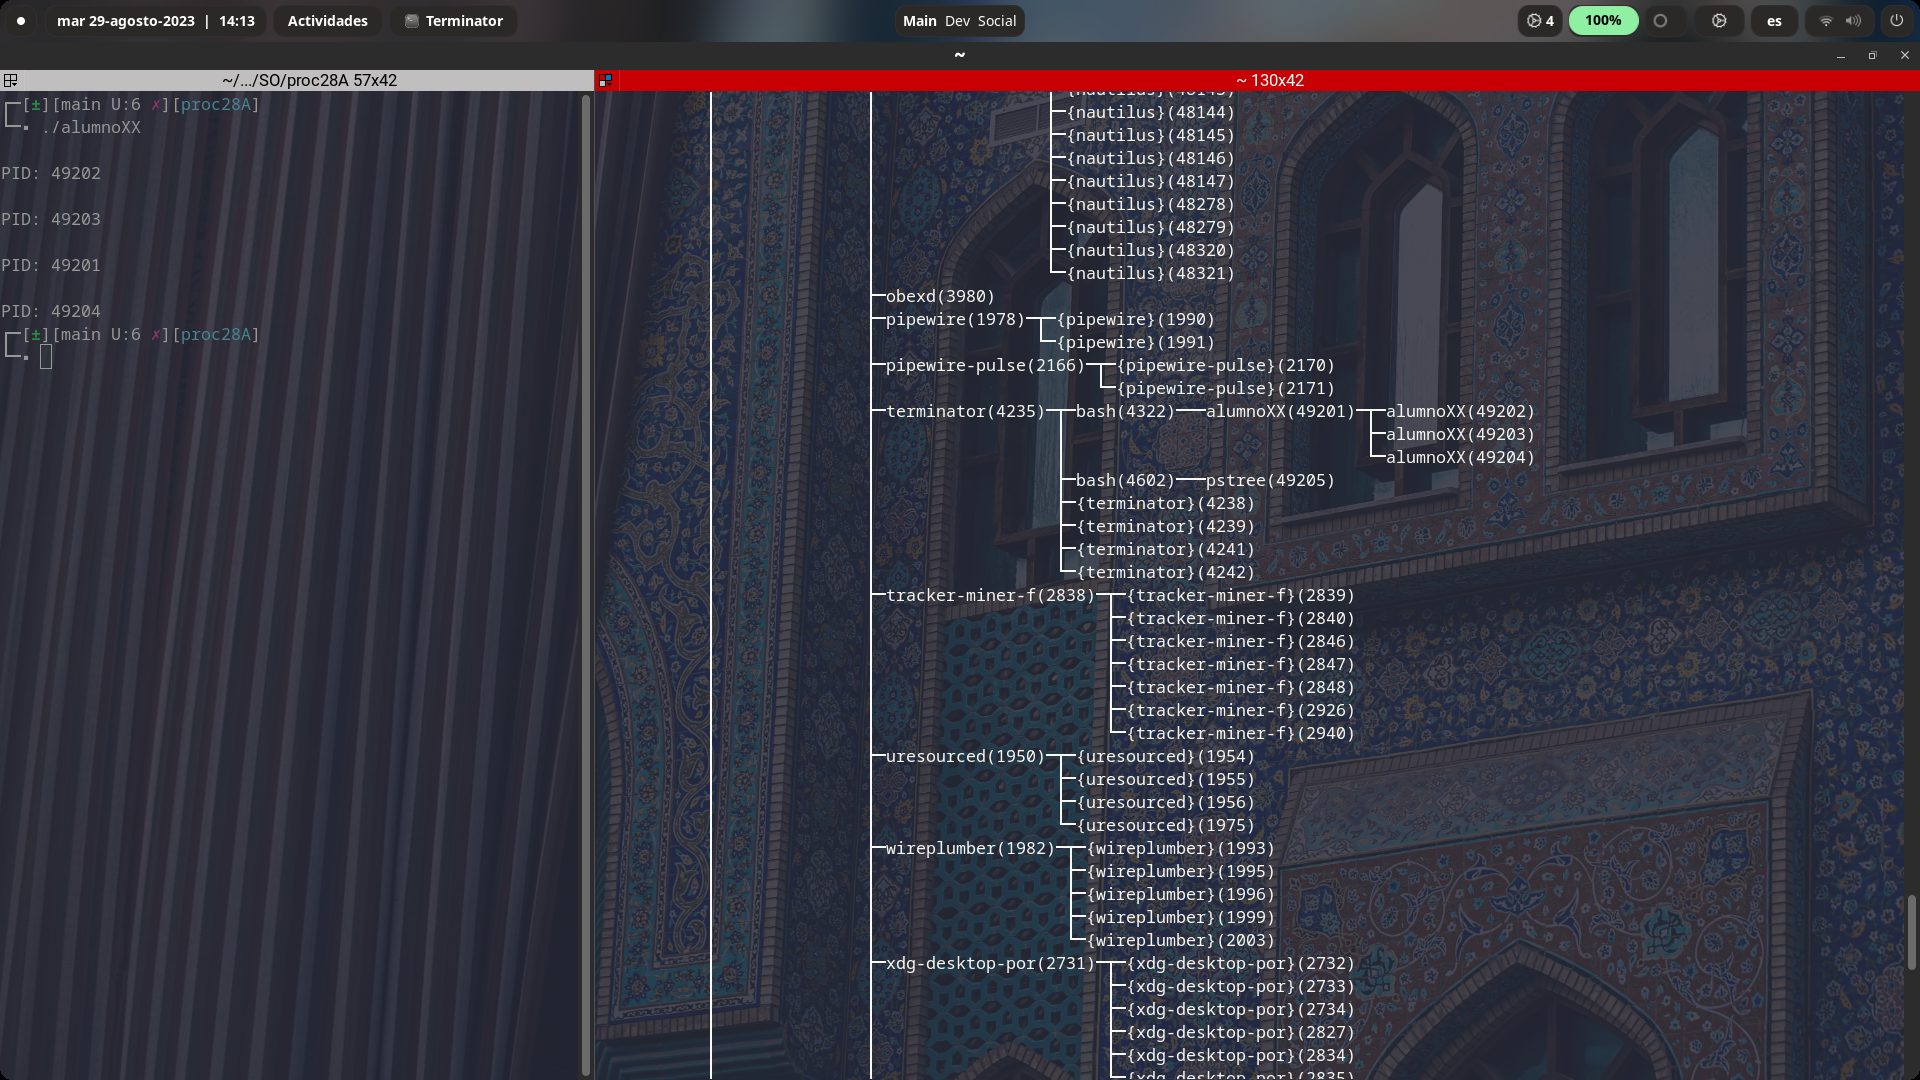
\includegraphics[width=\linewidth]{p6.png}
  \caption{Ejecución y árbol de procesos}
  \label{img:p6}
\end{figure}
\\\\
Por otro lado, en caso de que quisiéramos ejecutar un código de estos con la llamada a sistema \textbf{'wait()'} que hace unos cambios en el código, donde al quitar las instrucciones comentadas nos produce los siguientes resultados. 
\begin{figure}
\centering
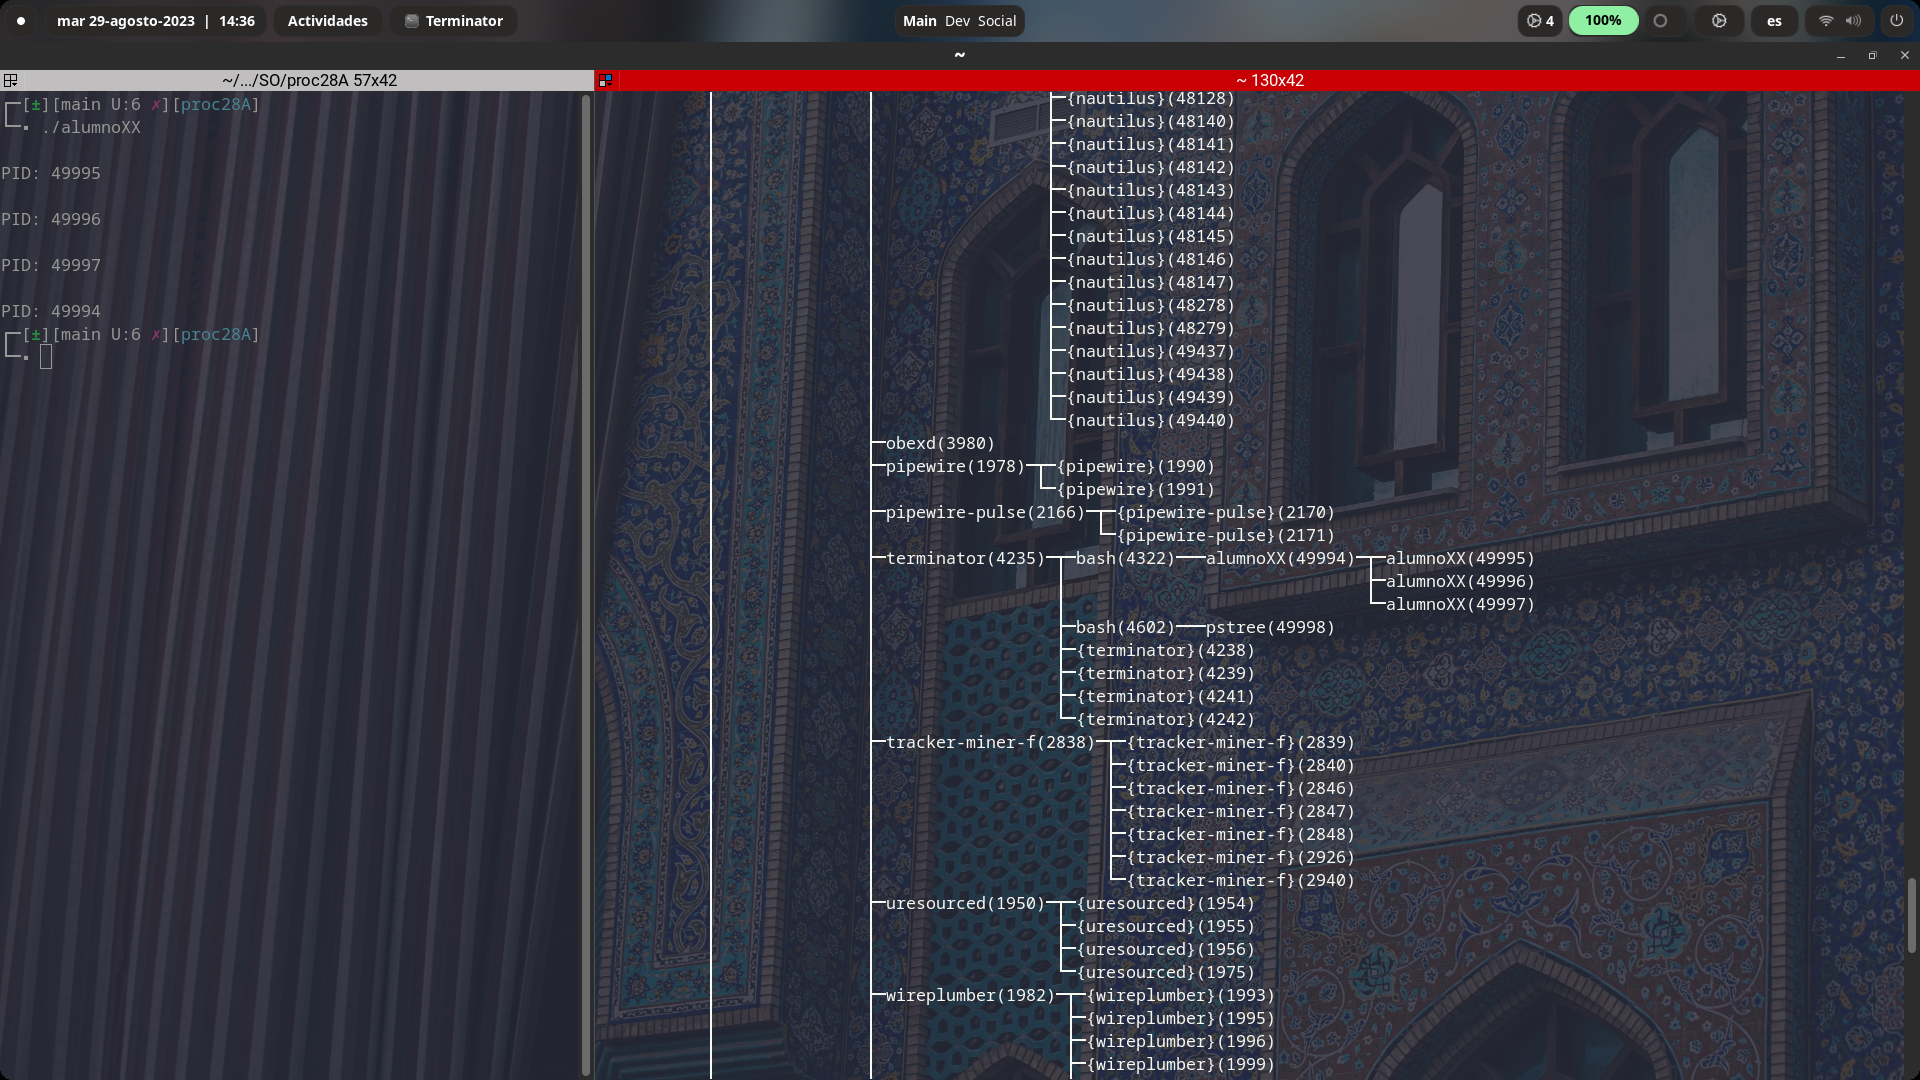
\includegraphics[width=\linewidth]{p6v2.png}
\caption{Ejecución y árbol de procesos con \textbf{wait()}}
\label{img: p6v2}
\end{figure}
\begin{figure}
\centering
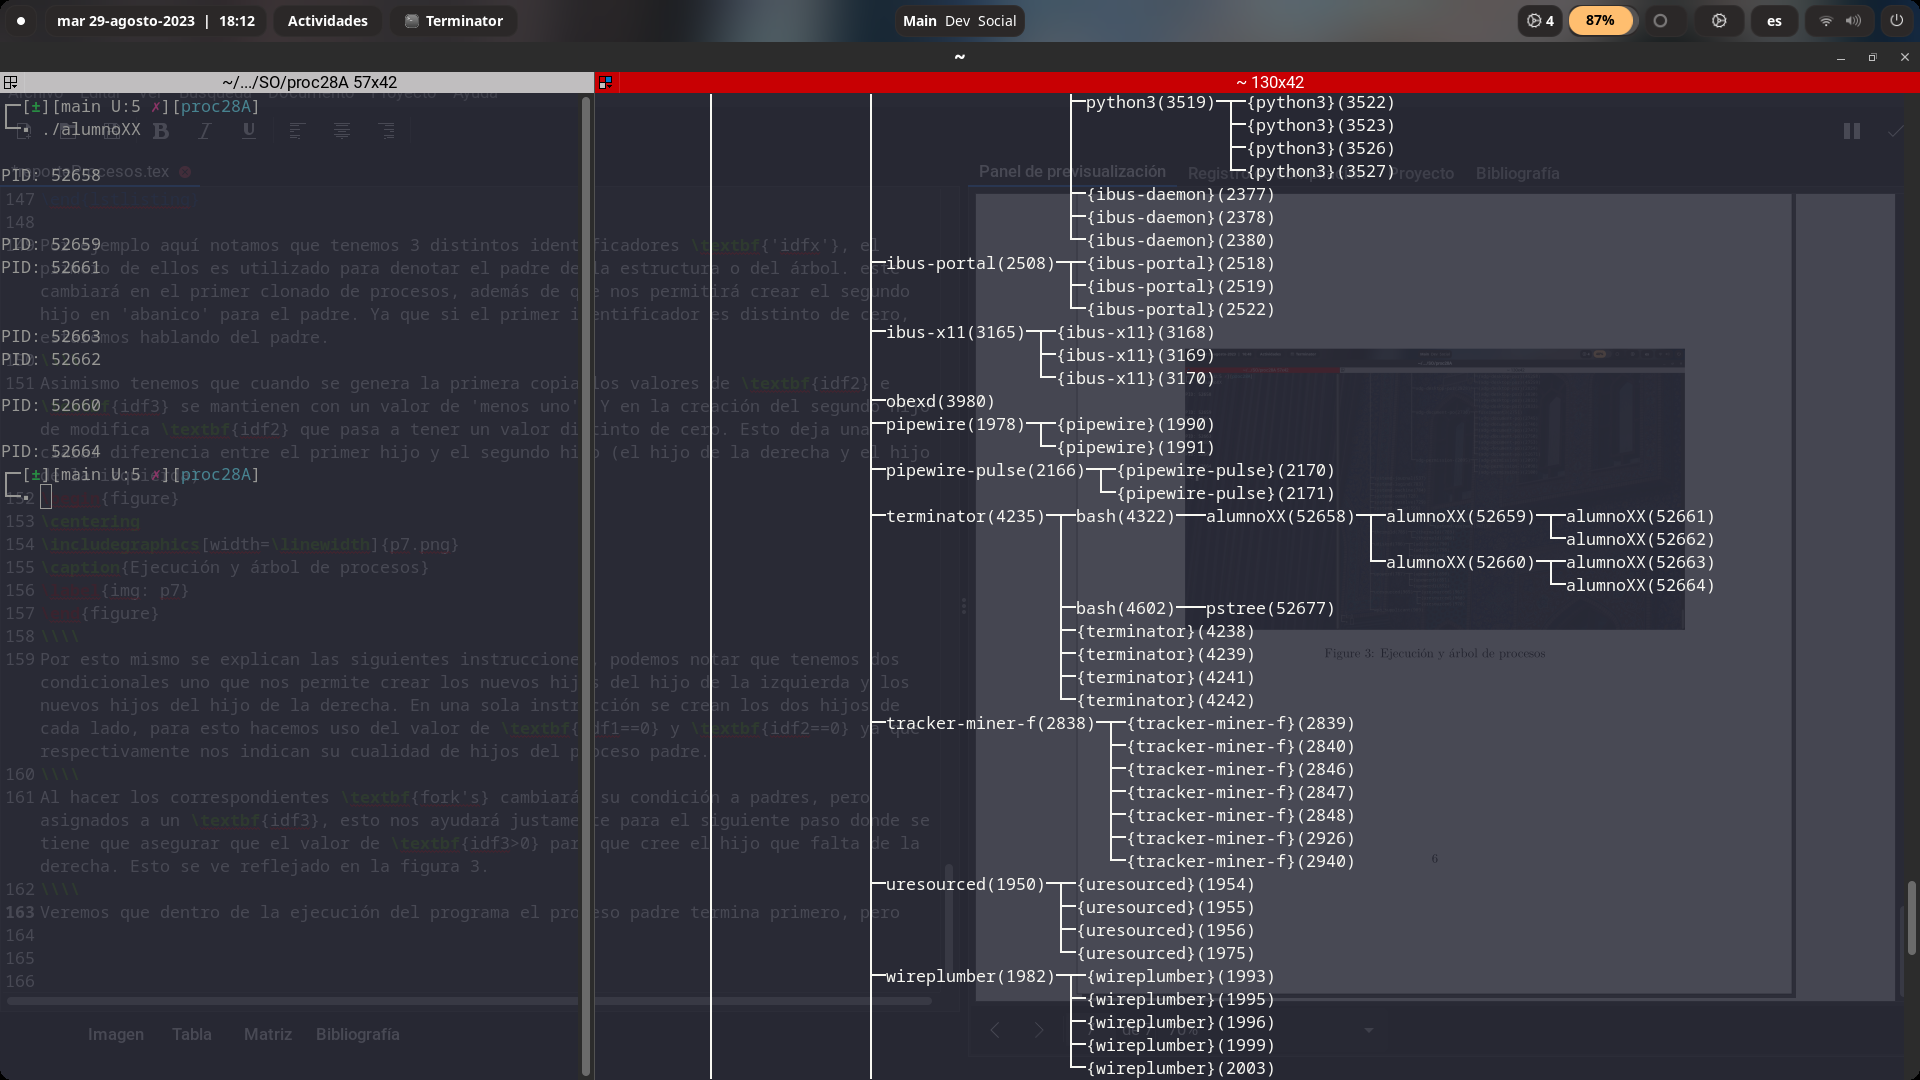
\includegraphics[width=\linewidth]{p7.png}
\caption{Ejecución y árbol de procesos}
\label{img: p7}
\end{figure}
\\\\
Podemos notar como claramente el proceso padre termina yendo hasta el final ya que por obvias razones ya que eso es lo que hace la llamada al sistema \textbf{wait()} espera a que los procesos hijos terminen de ejecutar para que el padre termine de ejecutar. 
\\\\
Esto no fue necesario para ninguna de las dos situaciones, nunca necesitamos como tal que el proceso padre esperará a que los hijos terminarán de ejecutar, pero se me ocurren un par de situaciones en los que sería conveniente que el proceso padre si lo hiciera, como puede ser el caso de un proceso hijo que recupere datos y sean necesarios antes de que el padre pase a las siguientes instrucciones.
\\\\
Otro punto a destacar es que aquí al tener procesos no tan caóticos es sencillo observar porque los procesos están terminando unos antes que otros. Pero la realidad es que la pelea que hacen los procesos por los recursos pueden ocurrir de muchas formas, podemos asumir que cualquier proceso podría terminar primero que otro cualquier proceso, obviamente sin usar la llamada a sistema \textbf{wait()}.
\\\\
\textbf{Segunda Estructura} 
\\
Para este caso tendremos muchas variables que nos ayudarán a distinguir entre padre de toda la estructura, padres del primer nivel e hijos que se encuentran en el último nivel. 

\begin{lstlisting}
#include <stdio.h>
#include <unistd.h>
#include <sys/types.h>

int main(){
  int idf1=-1, idf2=-1, idf3=-1;

  idf1=fork();
  if(idf1>0){
    idf2=fork();
  }
  if(idf1==0){
    idf3=fork();
    if(idf3>0){
      fork();
    }
  }
  if(idf2==0){
    idf3=fork();
    if(idf3>0){
      fork();
    }
  }
  printf("\nPID: %d\n", getpid());
  sleep(15);
  return 0;
}
\end{lstlisting}

Por ejemplo aquí notamos que tenemos 3 distintos identificadores \textbf{'idfx'}, el primero de ellos es utilizado para denotar el padre de la estructura o del árbol. este cambiará en el primer clonado de procesos, además de que nos permitirá crear el segundo hijo en 'abanico' para el padre. Ya que si el primer identificador es distinto de cero, estaremos hablando del padre. 
\\\\
Asimismo tenemos que cuando se genera la primera copia los valores de \textbf{idf2} e \textbf{idf3} se mantienen con un valor de 'menos uno'. Y en la creación del segundo hijo de modifica \textbf{idf2} que pasa a tener un valor distinto de cero. Esto deja una clarar diferencia entre el primer hijo y el segundo hijo (el hijo de la derecha y el hijo de la izquierda). 
\\\\
Por esto mismo se explican las siguientes instrucciones, podemos notar que tenemos dos condicionales uno que nos permite crear los nuevos hijos del hijo de la izquierda y los nuevos hijos del hijo de la derecha. En una sola instrucción se crean los dos hijos de cada lado, para esto hacemos uso del valor de \textbf{idf1==0} y \textbf{idf2==0} ya que respectivamente nos indican su cualidad de hijos del proceso padre. 
\\\\
Al hacer los correspondientes \textbf{fork's} cambiarán su condición a padres, pero asignados a un \textbf{idf3}, esto nos ayudará justamente para el siguiente paso donde se tiene que asegurar que el valor de \textbf{idf3>0} para que cree el hijo que falta de la derecha. Esto se ve reflejado en la figura 3. 
\\\\
Veremos que dentro de la ejecución del programa el proceso padre termina primero, pero no necesariamente los hijos terminarán primero que sus hijos, como bien dijimos antes es un concurso por los recursos de la computadora, entonces cualquiera que sea puede terminar primero y por razones distintas.
\\\\
\textbf{Tercera Esctructura}
\\
La siguiente estructura es un caso particular del caso anterior, donde solamente existe una rama, por lo que generar el código es muy sencillo, ya que solamente tenemos que quitar una parte del código anterior, justo donde se crea la rama derecha. Esto es. 
\begin{lstlisting}
#include <stdio.h>
#include <unistd.h>
#include <sys/types.h>

int main(){
  int idf1=-1, idf2=-1, idf3=-1;

  idf1=fork();
  if(idf1>0){
    idf2=fork();
  }
  if(idf1==0){
    idf3=fork();
    if(idf3>0){
      fork();
    }
  }
  printf("\nPID: %d\n", getpid());
  sleep(15);
  return 0;
}
\end{lstlisting}
De igual manera podríamos hacer que se llenará la rama del otro lado, simplemente tendríamos que cambiar el \textbf{idf1} dentro del \textit{if} por un \textbf{idf2} que de hecho es el hijo de la derecha. Podemos ver los resultados de ello en la figura 4.
\begin{figure}
\centering
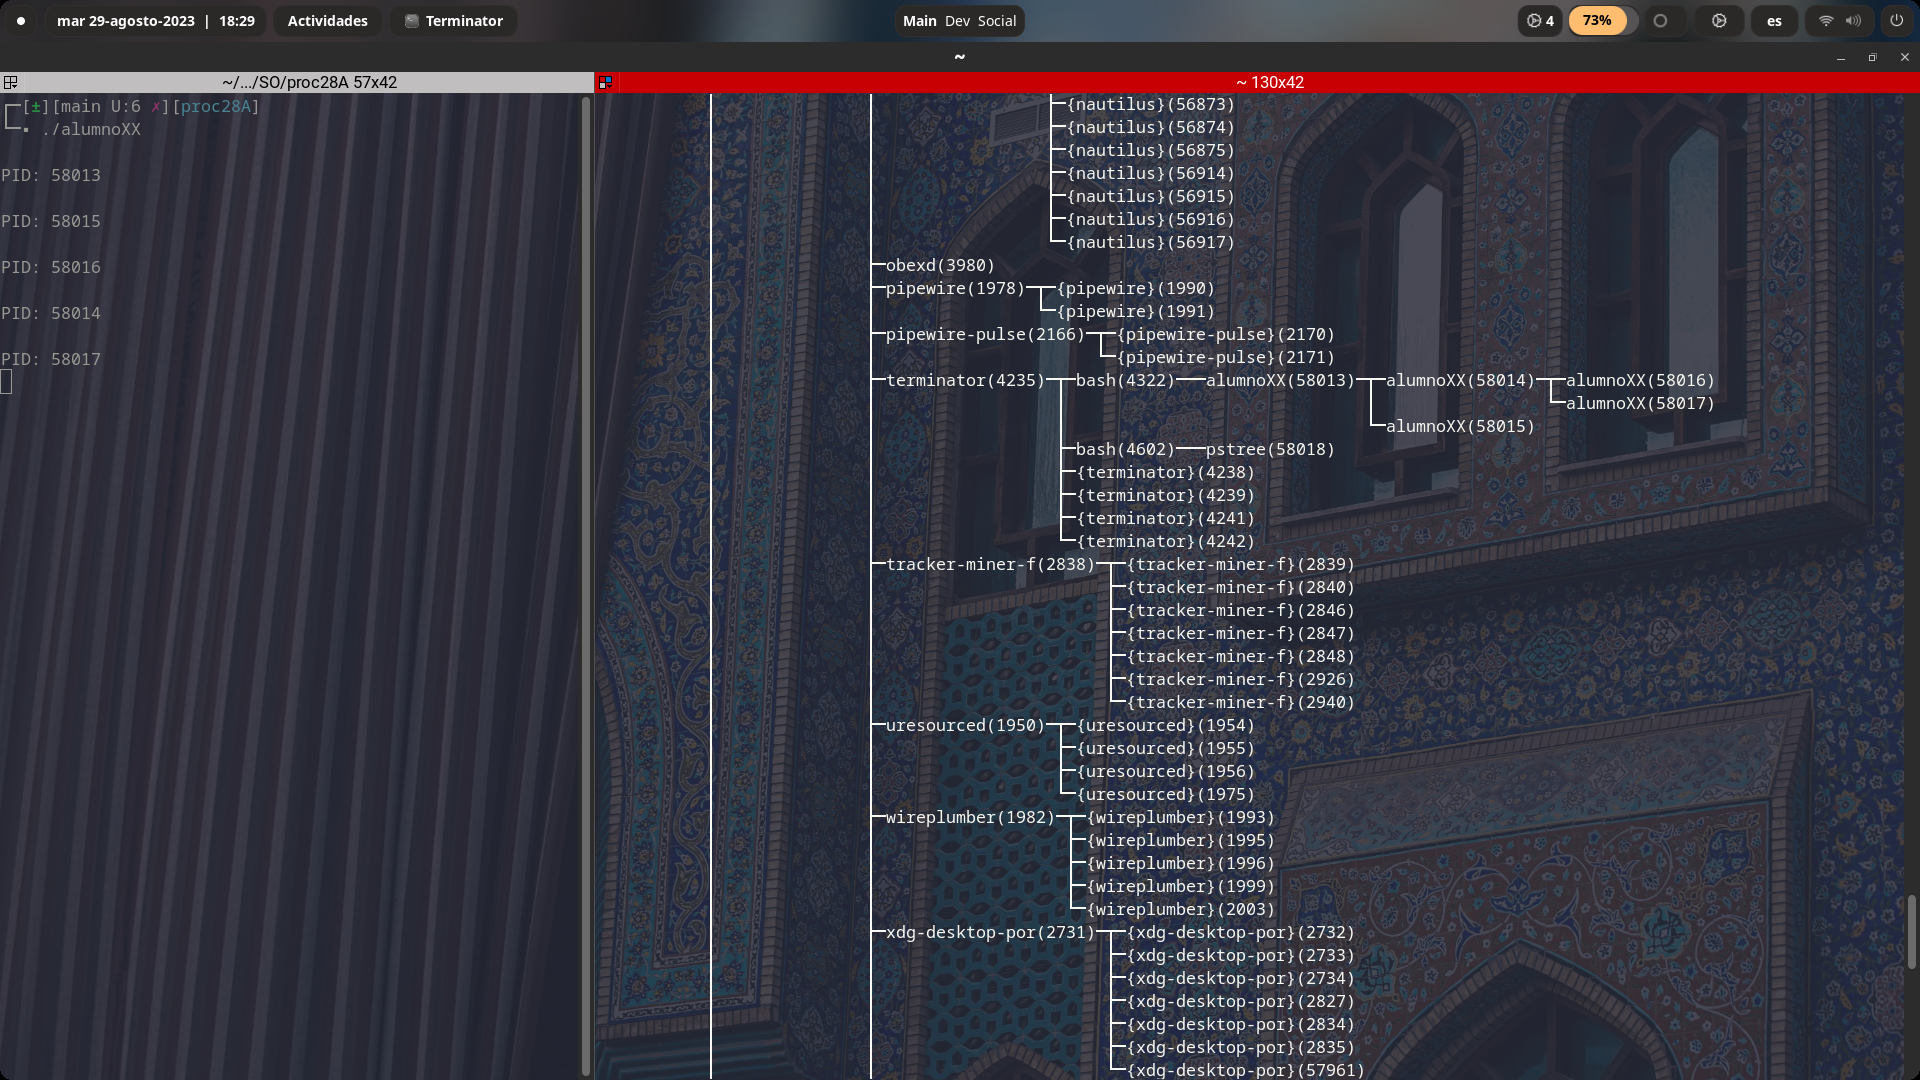
\includegraphics[width=\linewidth]{p8.png}
\caption{Ejecución y árbol de procesos}
\label{img: p8}
\end{figure}
\\\\
Notemos que el proceso padre así como su izquierdo terminan primero, luego le siguen los hijos del hijo derecho del proceso padre y por último el antes mencionado, de nuevo podemos ver como es que los procesos pelean por los recursos y depende de su forma de creación y en que posición del código sean duplicados para terminar. 
\end{document}